% --- Dataset ---

\begin{tframe}{Dataset}

Il dataset che contiene un totale di 12 dispositivi, che includono smartphone e tablet, di diverse case produttrici e modelli.

\vspace{0.1in}

In particolare i modelli in nostro possesso sono: un Galaxy S3, due Galaxy S3 mini, un Galaxy S4 mini, un Galaxy Tab 3, un Galaxy Tab, un Galaxy Trend Plus, un Huawei G6, un Ipad 2, un Ipad mini, un Iphone 4S, un Iphone 5. 

\vspace{0.1in}

Di tutti questi dispositivi siamo in possesso di immagini direttamente acquisite (immagini naturali) e delle stesse immagini ma caricate e scaricate da Facebook.


\end{tframe}

% --- Threshold ---

\begin{tframe}{Threshold}

La condizione di stop per l'algoritmo di clustering Normalized Cuts dipende dalla verifica di stabilità del taglio realizzato.

\vspace{0.1in}

Due diversi approcci sono stati confrontati:
\begin{itemize}
\item Comparare il valore di $Ncut(A, B)$ ad una soglia $T_{k}$ predefinita, come prevede l'implementazione originale dell'algoritmo.
\item Calcolare un coefficiente di aggregazione [1] per ciascuna delle partizioni ottenute e confrontare tale valore per una soglia $T_{k}$ predefinita, calcolato come segue: $AC(k) = \frac{1}{N_{k}} \sum_{i, j} w_{ij}$, ovvero il valore medio dei pesi associati ai nodi che appartengono alla partizione $k$.
\end{itemize}

\vspace{0.1in}

In entrambi i casi, la soglia è stata determinata attraverso uno studio dei valori di TPR e FPR, rispetto ad un groundtruth, al variare della soglia stessa.

\end{tframe}

\begin{tframe}{Threshold}

In generale, è stata scelta la soglia per la quale è minimo il valore di FPR, poiché la priorità è minimizzare il numero di falsi positivi all'interno dei clusters. A partire da questi, infatti, verranno calcolate le fingerprints.

\vspace{0.1in}

Tale studio è stato effetuato sia per le immagini naturali che per le immagini scaricate da Facebook. Sono stati considerati tutti e 12 i dispositivi, utilizzando 50 immagini da ciascuno.

\end{tframe}

\begin{tframe}{Threshold}

\begin{figure}[h]
\begin{center}
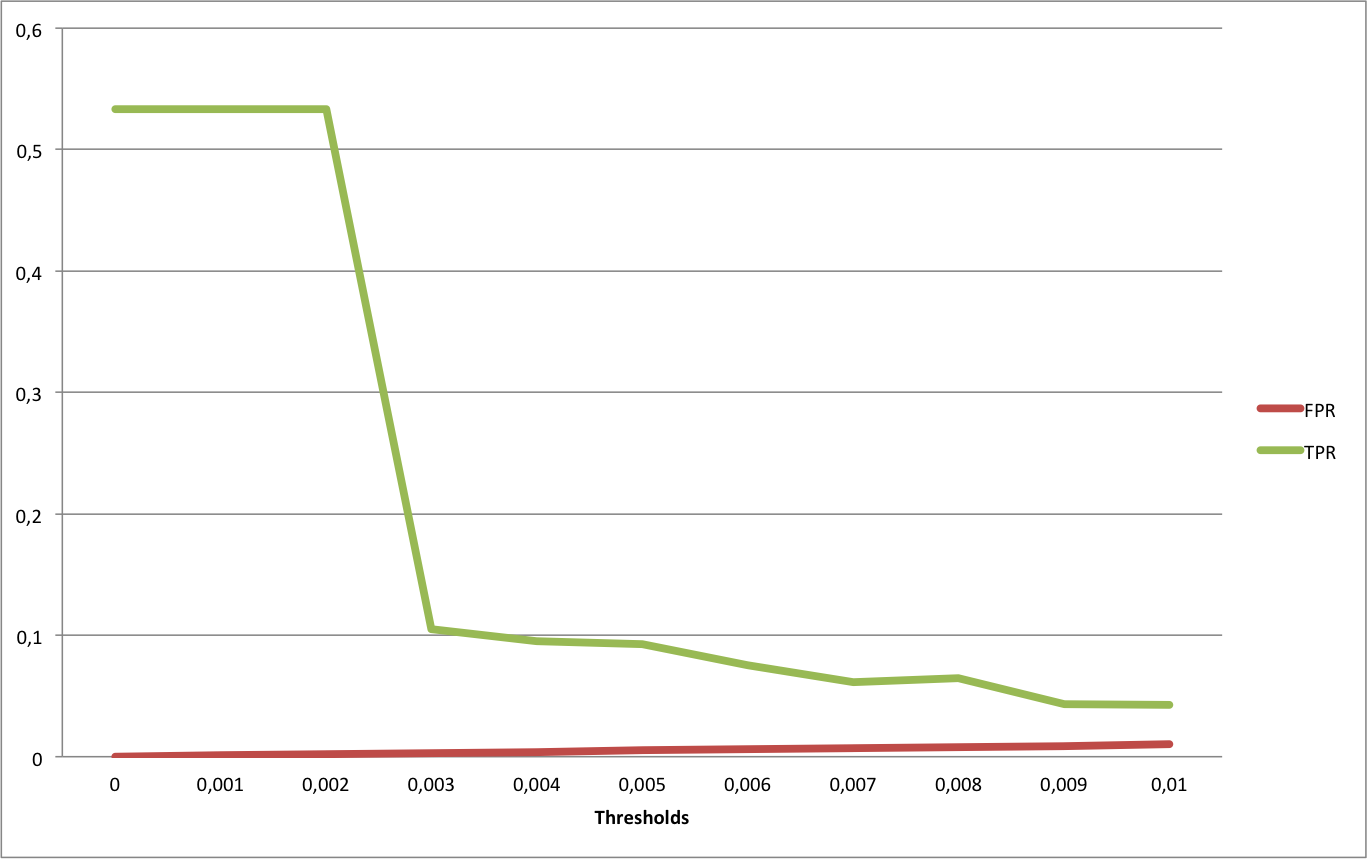
\includegraphics[width=0.8\textwidth]{../images/soglia_imgnat_AC.png}
\end{center}
  \caption{Valori di TPR e FPR al variare della soglia per le immagini naturali acquisite direttamente dai dispositivi. Metodo con coefficiente di aggregazione.}
\label{fig:soglia AC}
\end{figure}

\end{tframe}

\begin{tframe}{Threshold}

\begin{figure}[h]
\begin{center}
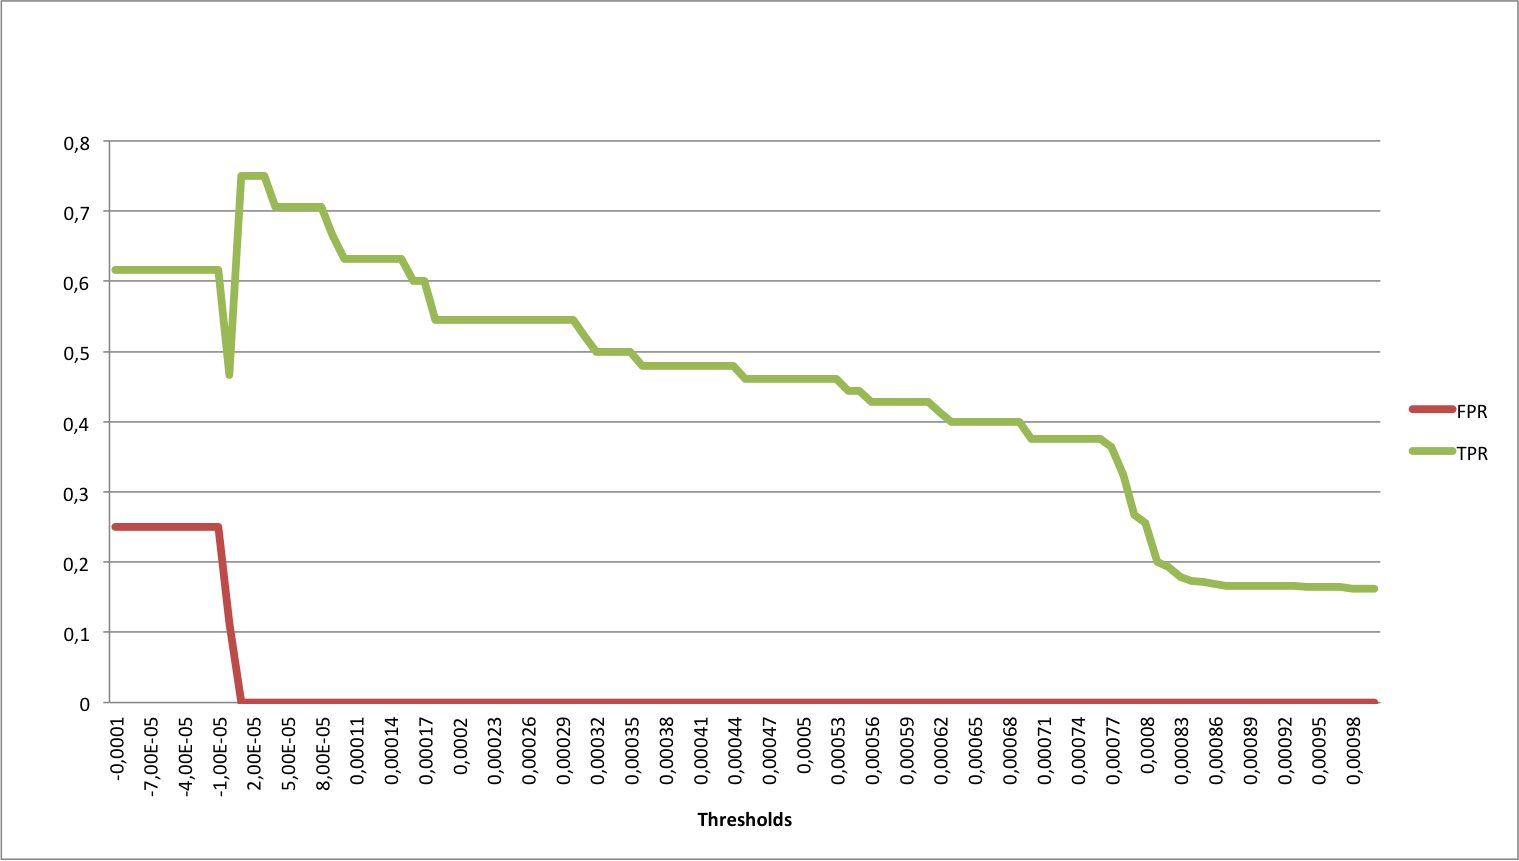
\includegraphics[width=0.8\textwidth]{../images/soglia_imgnat_NC.png}
\end{center}
  \caption{Valori di TPR e FPR al variare della soglia per le immagini naturali acquisite direttamente dai dispositivi. Metodo che considera i valori di $Ncuts$.}
\label{fig:soglia AC}
\end{figure}

\end{tframe}

\begin{tframe}{Threshold}

\begin{figure}[h]
\begin{center}
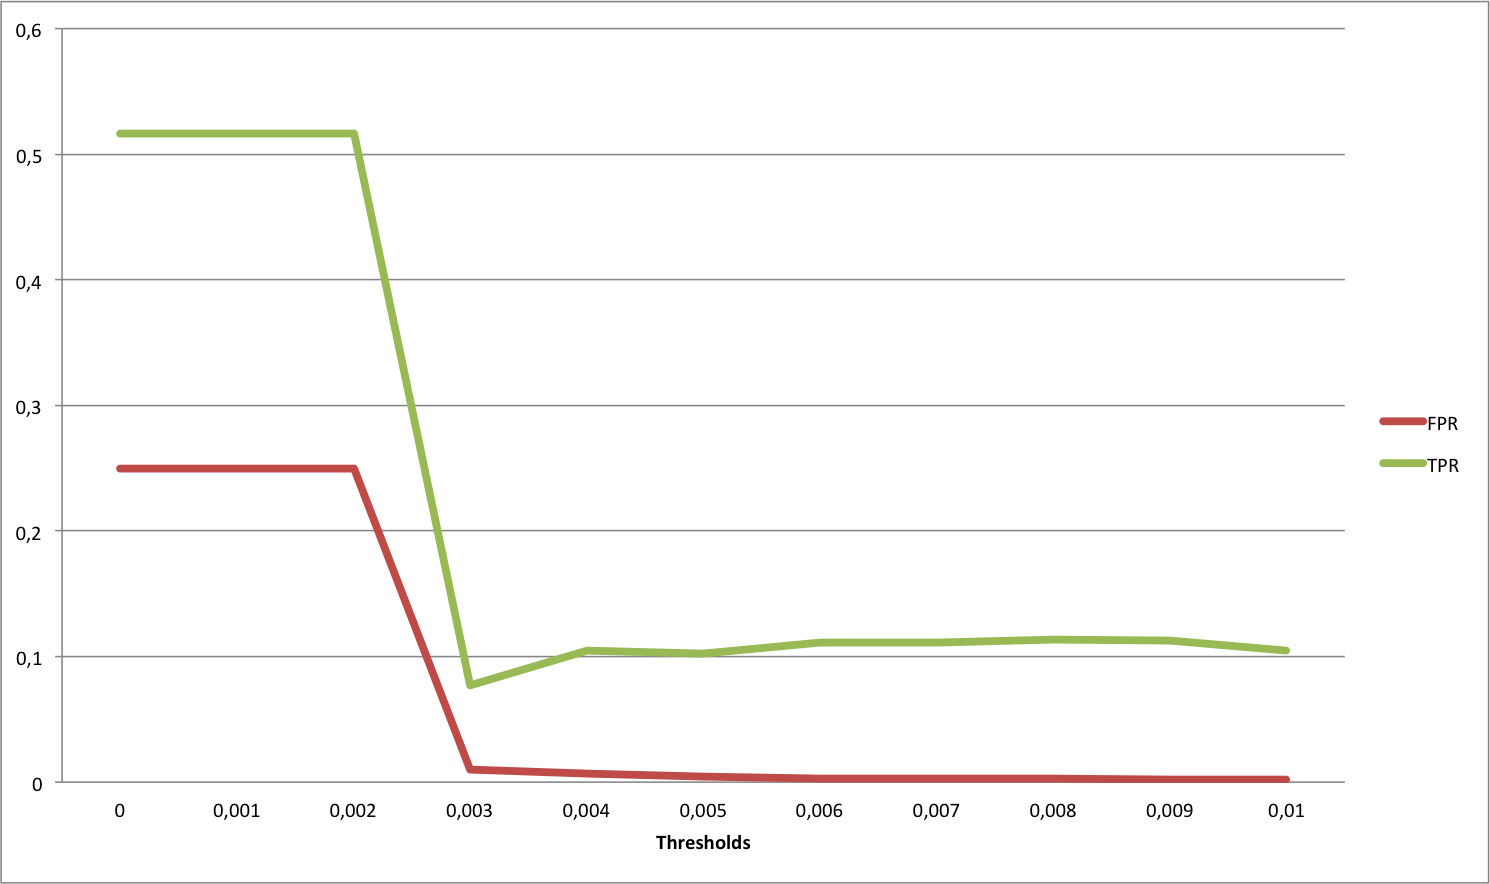
\includegraphics[width=0.8\textwidth]{../images/soglia_imgnat_fb_AC.png}
\end{center}
  \caption{Valori di TPR e FPR al variare della soglia per le immagini scaricate da Facebook. Metodo con coefficiente di aggregazione.}
\label{fig:soglia AC}
\end{figure}

\end{tframe}

\begin{tframe}{Threshold}

\begin{figure}[h]
\begin{center}
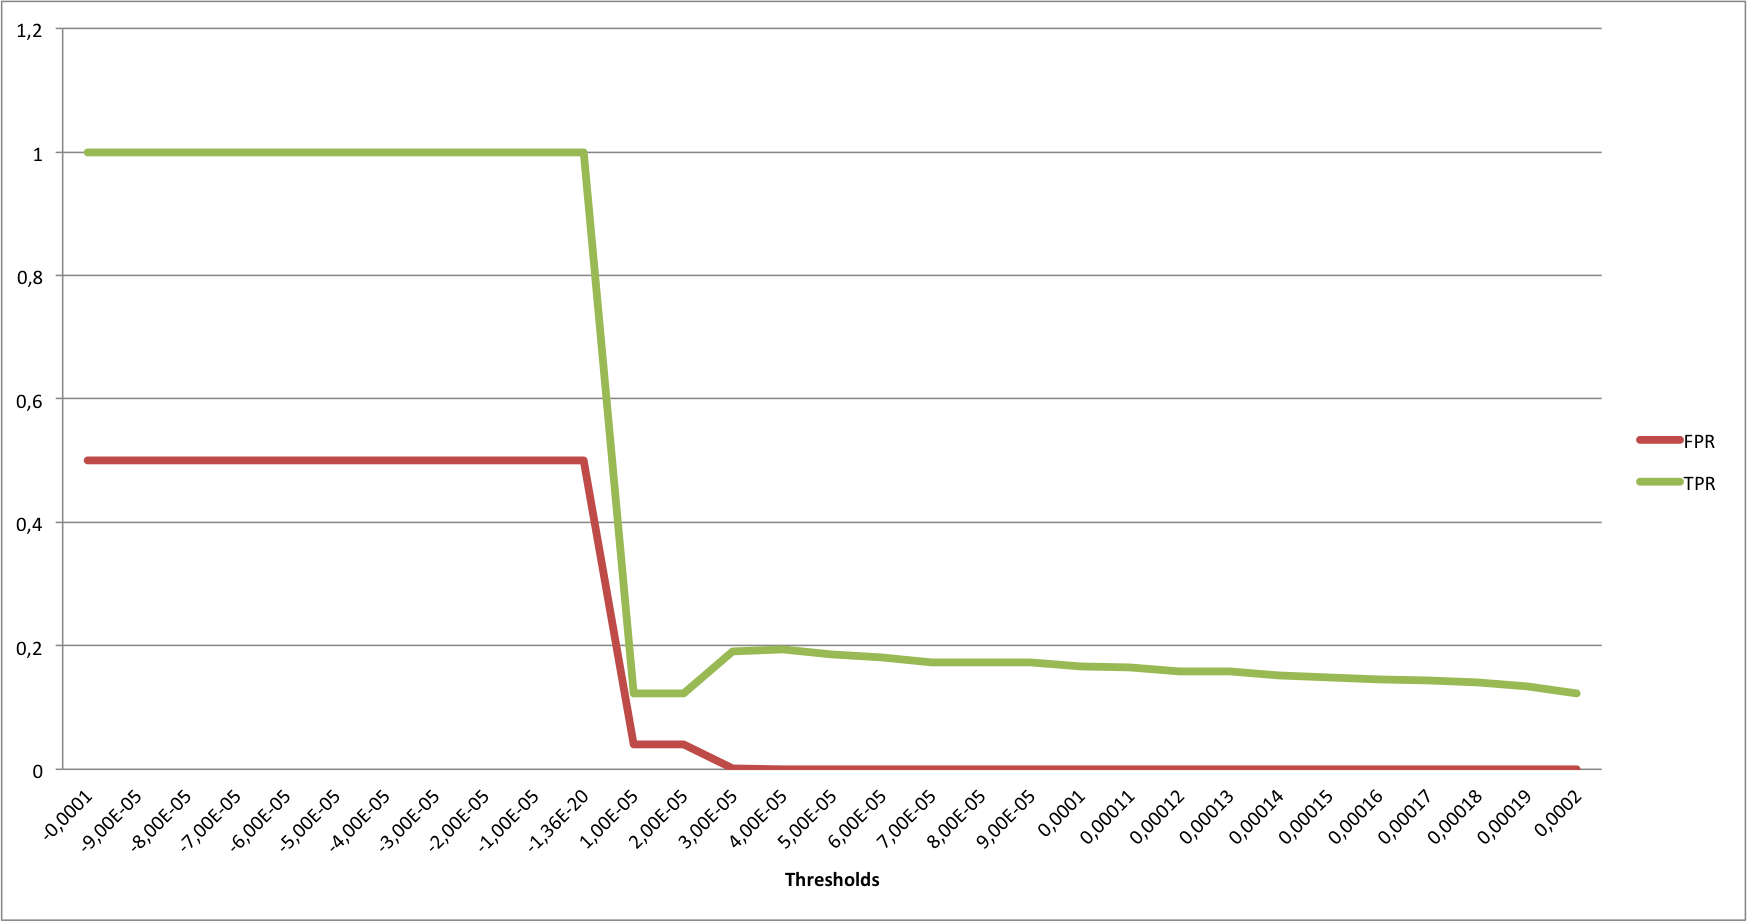
\includegraphics[width=0.8\textwidth]{../images/soglia_imgnat_fb_NC.png}
\end{center}
  \caption{Valori di TPR e FPR al variare della soglia per le immagini scaricate da Facebook. Metodo che considera i valori di $Ncuts$.}
\label{fig:soglia AC}
\end{figure}

\end{tframe}

\begin{tframe}{Threshold}

Come mostrato nei grafici, i valori di TPR e FPR sono consistentemente migliori per il metodo che considera i valori di $Ncut(A, B)$. Per tale motivo è stato scelto di usare tale metodo, ovvero l'approccio standard dell'algoritmo Normalized Cuts.

\vspace{0.1in}

La soglia ottimale per le immagini naturali è pari a $10^{-5}$, corrispondente a TPR = 0.75 e FPR = 0.

\vspace{0.1in}

Invece, la soglia ottimale per le immagini scaricate da Facebook è pari a $4*10^{-5}$, corrispondente a TPR = 0.2 e FPR prossima allo zero.

\end{tframe}

% --- Esperimenti ---

\begin{tframe}{Esperimenti}

Il dataset è stato diviso in tre insiemi da 4, 5 e 6 dispositivi. Gli esperimenti per la fase di validazione sono stati eseguiti sia per le immagini naturali che per le immagini scaricate da Facebook.

\begin{table}[ht]
\centering % used for centering table
\scalebox{0.6}{
\begin{tabular}{c c l c} % centered columns (4 columns)
\hline\hline %inserts double horizontal lines
Test set & No images & Brand and Model & No images per camera \\ [0.5ex] % inserts table
%heading
\hline % inserts single horizontal line
A & 300 & Galaxy S3 & 50\\ % inserting body of the table
& & Galaxy S3 mini & 50\\
& & Galaxy S3 mini & 50\\
& & Galaxy S4 mini & 50\\
& & Galaxy Tab 3 & 50\\
& & Galaxy Tab & 50\\
\\
B & 250 & Huawei G6 & 50\\
& & Ipad 2 & 50\\
& & Ipad mini & 50\\
& & Iphone 4S & 50\\
& & Iphone 5 & 50\\
\\
C & 200 & Galaxy Tab 3 & 50\\
& & Galaxy Tab & 50\\
& & Galaxy Trend Plus & 50\\
& & Huawei G6 & 50\\ [1ex] % [1ex] adds vertical space
\hline %inserts single line
\end{tabular}
}
\label{table:nonlin} % is used to refer this table in the text
\end{table}

\end{tframe}

\begin{tframe}{Esperimenti}

Innanzitutto, vengono prima mostrati i valori medi di TPR e FPR per i clusters calcolati nei vari esperimenti.

\begin{table}[ht]
\centering % used for centering table
\scalebox{0.8}{
\begin{tabular}{c l c c c} % centered columns (4 columns)
\hline\hline %inserts double horizontal lines
Test set & Type & No clusters & TPR & FPR \\ [0.5ex] % inserts table
%heading
\hline % inserts single horizontal line
A & Natural images & 8 & 0.750 & 0.000 \\ % inserting body of the table
B & Natural images & 7 & 0.714 & 0.000 \\
C & Natural images & 5 & 0.800 & 0.000 \\
\\
A & Facebook highres images & 20 & 0.298 & $10^{-4}$ \\ 
B & Facebook highres images & 12 & 0.333 & $10^{-5}$ \\
C & Facebook highres images & 12 & 0.294 & 0.004 \\ [1ex] % [1ex] adds vertical space
\hline %inserts single line
\end{tabular}
}
\label{table:nonlin} % is used to refer this table in the text
\end{table}

\end{tframe}

\begin{tframe}{Esperimenti}

Nelle slides seguenti verranno mostrati i risultati della fase di validazione per i vari esperimenti, sia per le immagini naturali che per le immagini scaricate da Facebook.

\vspace{0.1in}

Per la fase di validazione l'accuratezza è stata calcolata confrontando le associazioni con un groundtruth. Da ciascuna camera sono state utilizzate 20 immagini, non precedentemente usate nella fase di estrazione delle fingerprints.

\vspace{0.1in}

I risultati sono rappresentati tramite l'uso di matrici di confusione.

\end{tframe}

\begin{tframe}{Esperimenti}

\begin{figure}[h]
\begin{center}
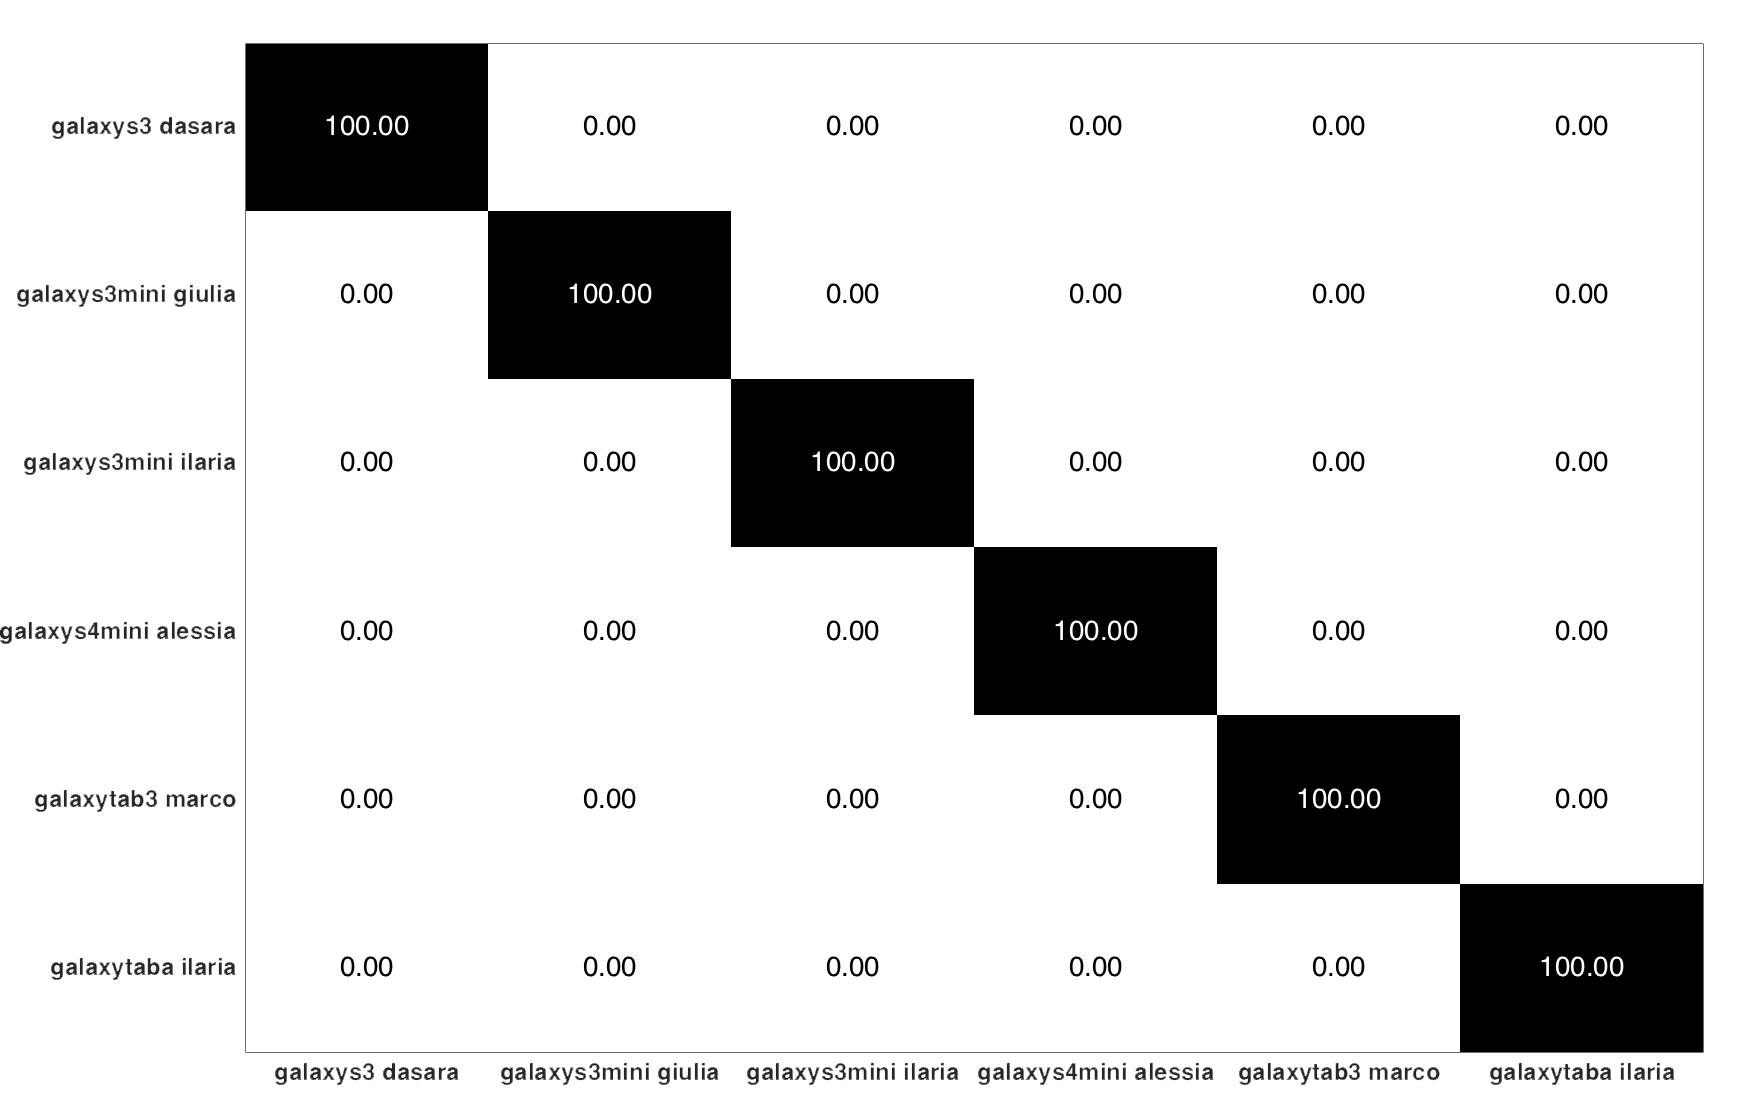
\includegraphics[width=0.75\textwidth]{../images/confusionmatrix_nat_6.png}
\end{center}
  \caption{Matrice di confusione per il caso delle immagini naturali usando 6 dispositivi.}
\label{fig:validation}
\end{figure}

\end{tframe}

\begin{tframe}{Esperimenti}

\begin{figure}[h]
\begin{center}
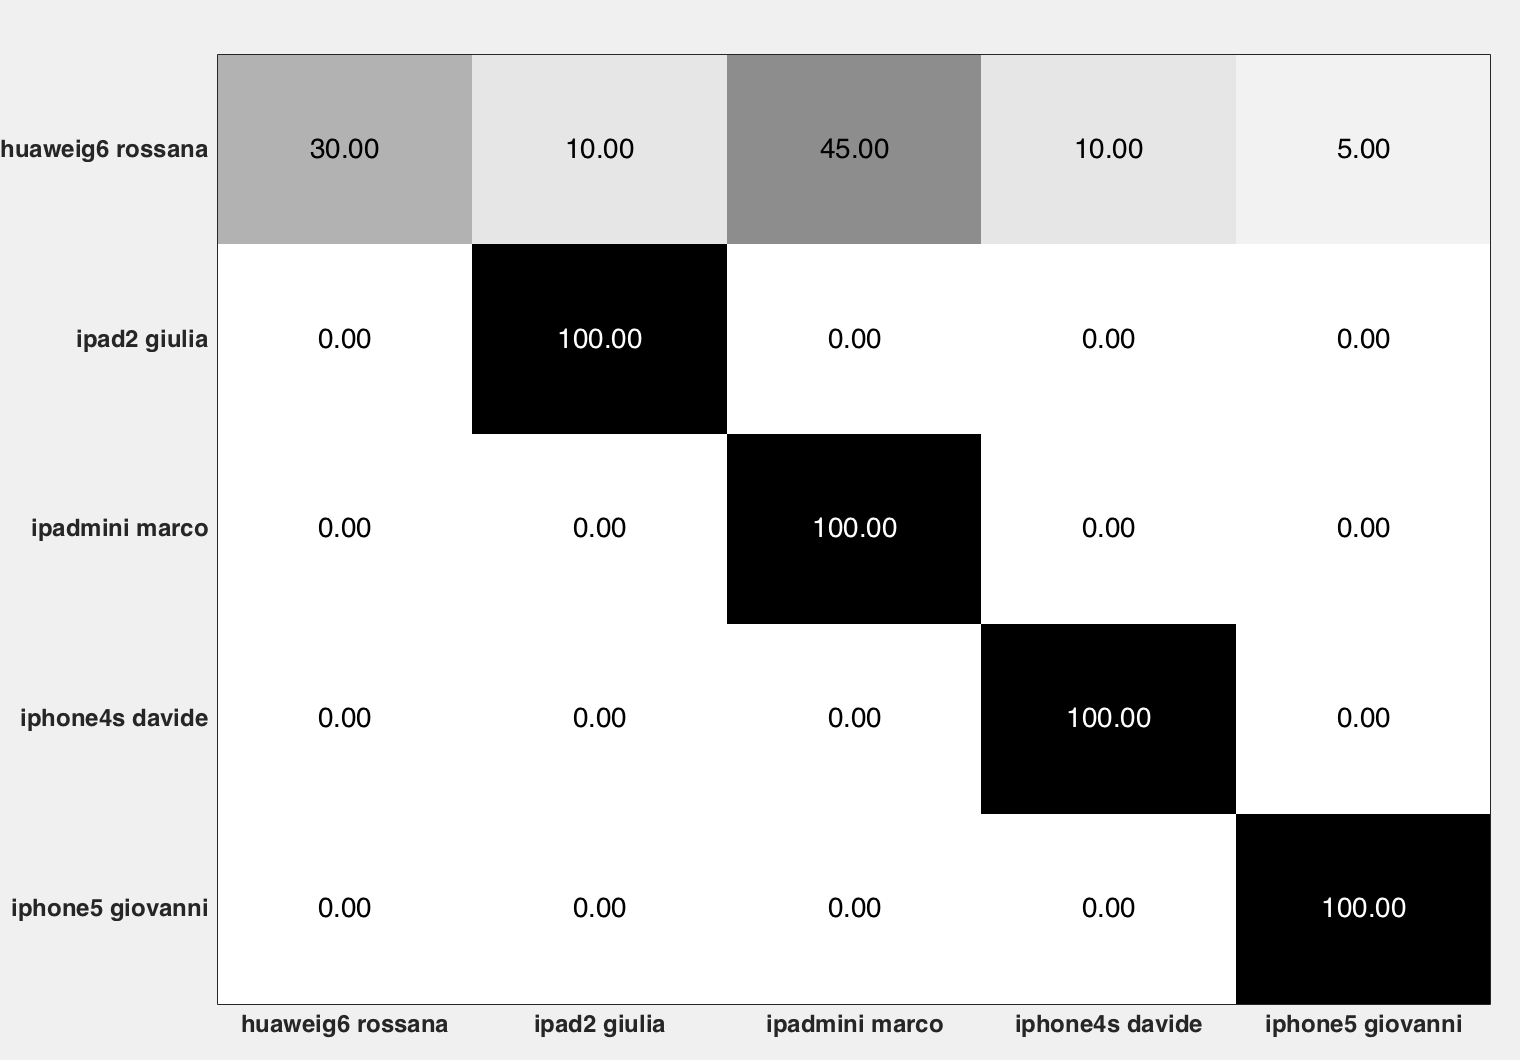
\includegraphics[width=0.75\textwidth]{../images/confusionmatrix_nat_5.png}
\end{center}
  \caption{Matrice di confusione per il caso delle immagini naturali usando 5 dispositivi.}
\label{fig:validation}
\end{figure}

\end{tframe}

\begin{tframe}{Esperimenti}

\begin{figure}[h]
\begin{center}
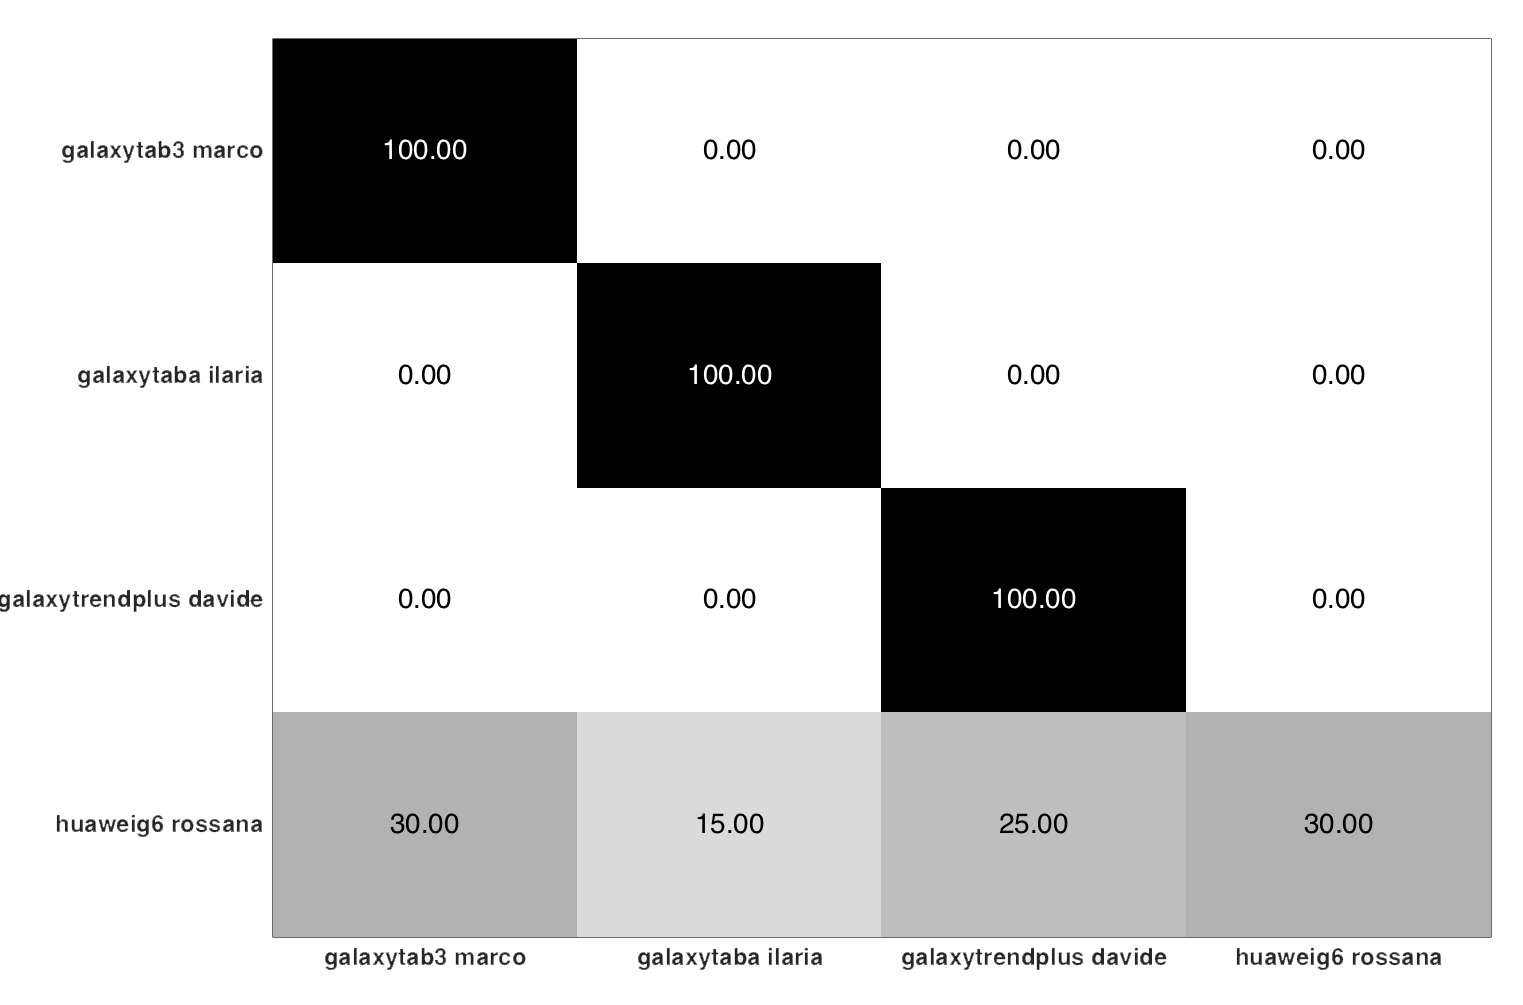
\includegraphics[width=0.75\textwidth]{../images/confusionmatrix_nat_4.png}
\end{center}
  \caption{Matrice di confusione per il caso delle immagini naturali usando 4 dispositivi.}
\label{fig:validation}
\end{figure}

\end{tframe}

\begin{tframe}{Esperimenti}

\begin{figure}[h]
\begin{center}
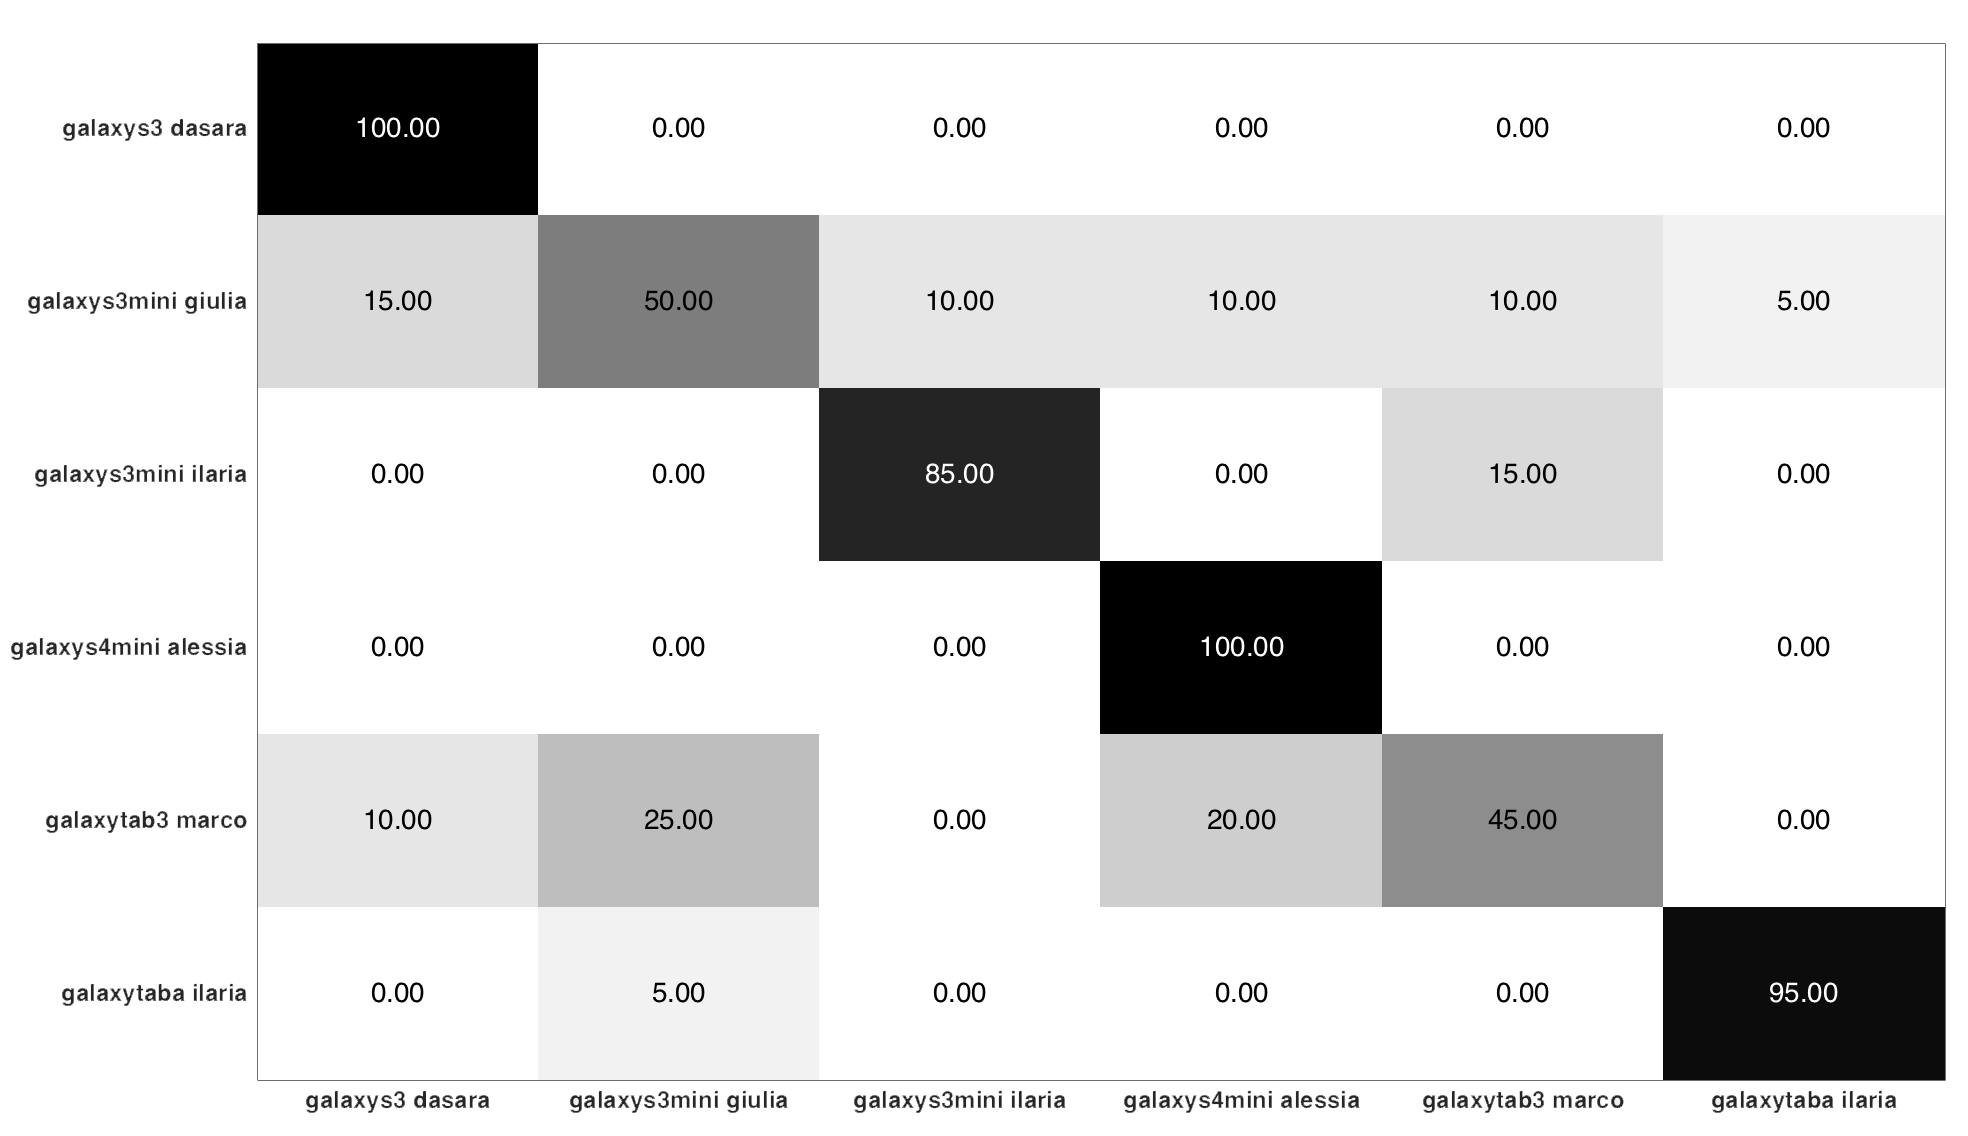
\includegraphics[width=0.75\textwidth]{../images/confusion_matrix_fb_highres_6.png}
\end{center}
  \caption{Matrice di confusione per il caso delle immagini scaricate da Facebook usando gli stessi 6 dispositivi del caso delle immagini naturali.}
\label{fig:validation}
\end{figure}

\end{tframe}

\begin{tframe}{Esperimenti}

\begin{figure}[h]
\begin{center}
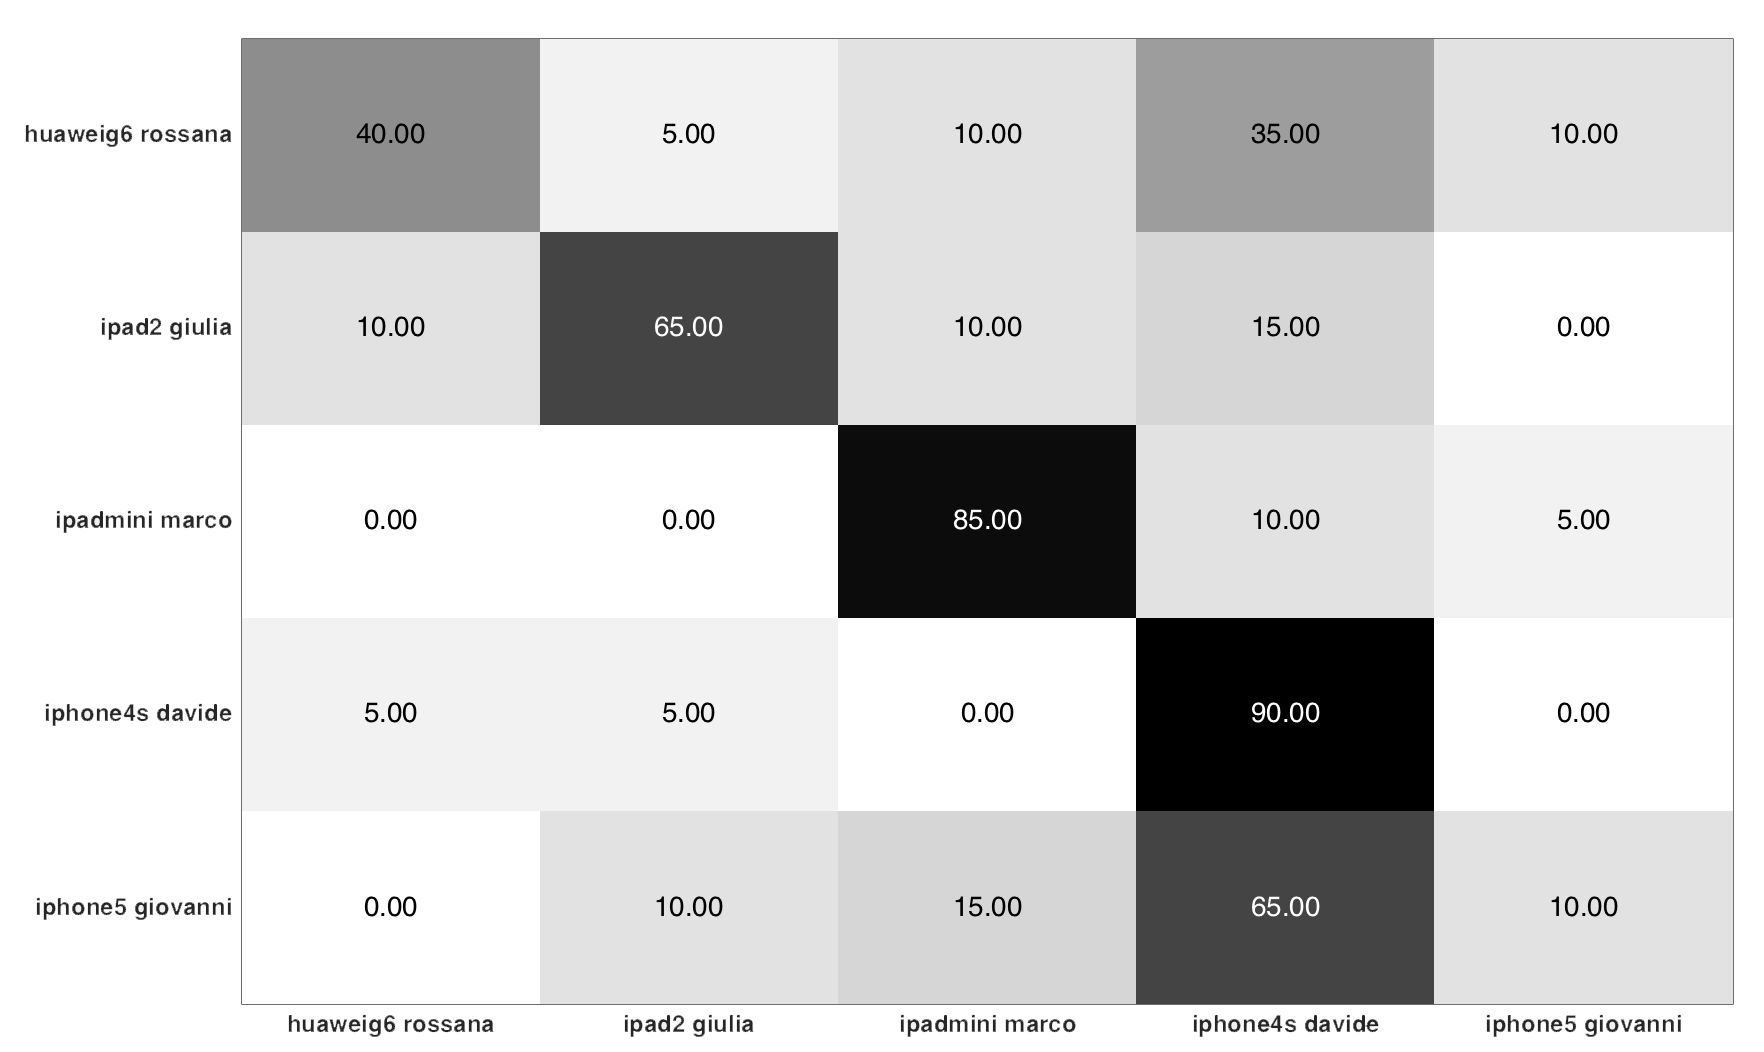
\includegraphics[width=0.75\textwidth]{../images/confusion_matrix_fb_highres_5.png}
\end{center}
  \caption{Matrice di confusione per il caso delle immagini scaricate da Facebook usando gli stessi 5 dispositivi del caso delle immagini naturali.}
\label{fig:validation}
\end{figure}

\end{tframe}

\begin{tframe}{Esperimenti}

\begin{figure}[h]
\begin{center}
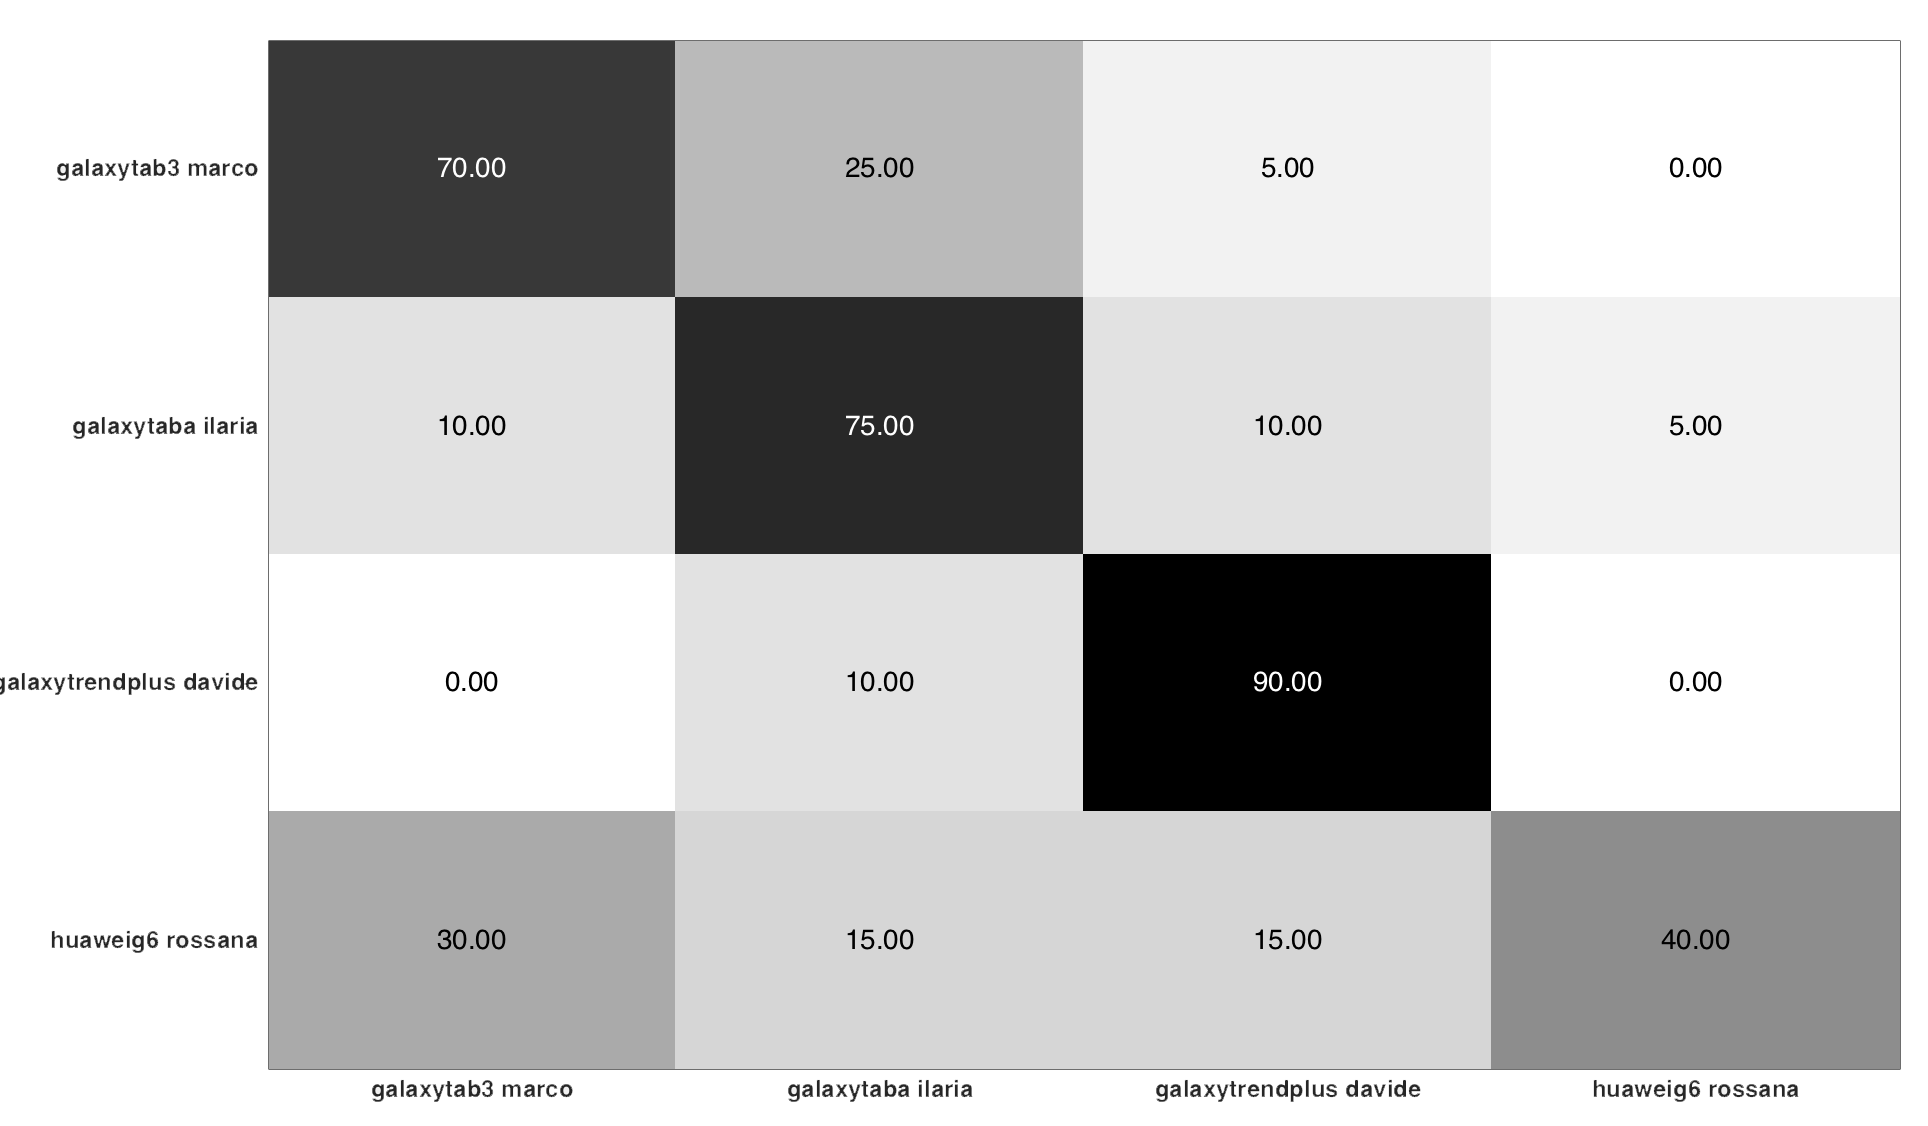
\includegraphics[width=0.75\textwidth]{../images/confusion_matrix_fb_highres_4.png}
\end{center}
  \caption{Matrice di confusione per il caso delle immagini scaricate da Facebook usando gli stessi 4 dispositivi del caso delle immagini naturali. }
\label{fig:validation}
\end{figure}

\end{tframe}

\begin{tframe}{Esperimenti}

Come mostrato dalle matrici di confusione, i risultati per le immagini naturali sono ottimi tranne che per il dispositivo Huawei G6.

\vspace{0.1in}

I risultati per le immagini scaricate da Facebook, invece, presentano risultati altalenanti con alcune camere con accuratezza di predizione molto alta (85\% o superiore) ad altre con accuratezza mediocre (circa 40-50\%). 

\vspace{0.1in}

Ciò è probabilmente dovuto al fatto che la compressione subita dalle immagini incide sulla qualità della PRNU estratta, ripercuotendosi così sulla PCE, utilizzata come misura di similarità, e quindi sul clustering. I valori medi di PCE sono infatti di un ordine di grandezza inferiore rispetto al caso delle immagini naturali.

\end{tframe}